\documentclass[jou,a4paper]{apa6}
\usepackage{enumitem}
\usepackage{fancyhdr}
\pagestyle{fancy}
\setlength{\headheight}{25pt}
\usepackage{hyperref}
\usepackage{url}
\usepackage{lastpage}
\usepackage[natbibapa]{apacite} 
\bibliographystyle{apacite}

\begin{document}

% JEMR Definitions
\newcommand{\jemrVolume}{x}
\newcommand{\jemrIssue}{y}
\newcommand{\jemrArticle}{z}
\newcommand{\jemrLastPage}{\pageref{LastPage}}
\newcommand{\jemrReceivedDate}{Mmm dd, 2016}
\newcommand{\jemrPublishedDate}{Mmm dd, 2016}
\newcommand{\jemrShortTitle}{``Ocular tremor'' in Parkinson's disease}
% JEMR-specific definitions

\setlist[itemize]{noitemsep, topsep=0pt}

\makeatletter
\renewcommand*{\addperi}[1]{#1.~}

\renewcommand{\section}{\@startsection {section}{1}{24pt}%
{12pt}{12pt}%
{\centering\normalfont\large}}

\renewcommand{\subsection}{\@startsection{subsection}{2}{0pt}%
{6pt}{6pt}%
{\normalfont\normalsize\itshape}}

\renewcommand{\subsubsection}{\@startsection{subsubsection}{3}{24pt}%
{\parskip}%
{-\parskip}%
{\normalfont\normalsize\itshape\bfseries\addperi}}

\makeatother

% header on first page
\fancypagestyle{plain}{%
\fancyhf{} % clear all header and footer fields
\fancyhead[L]{\small
Journal of Eye Movement Research\\
\jemrVolume(\jemrIssue):\jemrArticle, 1-\jemrLastPage}
\fancyfoot[C]{\thepage}
\renewcommand{\headrulewidth}{0pt}
\renewcommand{\footrulewidth}{0pt}}

% End of JEMR Definitions

\title{``Pervasive ocular tremor of Parkinson's'' is neither pervasive nor ocular nor uniquely parkinsonian.}
\fiveauthors
	{Michael R. MacAskill}
	{Daniel J. Myall}
	{Toni L. Pitcher}
	{Masayuki Watanabe}
	{Tim J. Anderson}
\fiveaffiliations
    {New Zealand Brain Research Institute,\\Christchurch, New Zealand\\
    Department of Medicine, University of Otago, Christchurch}
    {New Zealand Brain Research Institute,\\Christchurch, New Zealand}
    {New Zealand Brain Research Institute,\\Christchurch, New Zealand\\
    Department of Medicine, University of Otago, Christchurch}
	{New Zealand Brain Research Institute,\\Christchurch, New Zealand}
    {New Zealand Brain Research Institute,\\Christchurch, New Zealand\\
    Department of Medicine, University of Otago, Christchurch\\
    Department of Neurology, Christchurch Hospital}

\abstract{
A putative tremulous oscillation of the eyes has been proposed to provide the long-sought objective, sensitive and specific diagnostic sign for Parkinson's disease . Vigorous debate has ensued as to whether this ``ocular tremor'' is a real phenomenon or an artefact secondary to head motion. Contradictory arguments have centred on the capabilities of magnetic movement measurement technologies, with small numbers of illustrative cases presented to bolster either side. A large, definitive study able to either confirm or reject the original finding on a purely oculographic basis was required.
We examined 681 oculomotor recordings from a longitudinal study of 188 Parkinson's patients and 66 controls. Fourier analysis was used to detect oscillations not only in their raw pupil motion data but also in corneal reflection signals, which can correct for head motion.
We replicated the original authors' findings inasmuch as we detected oscillations in raw pupil position data that often occurred in their reported frequency range of 5.7 $\pm$ 3 Hz. They were not, however, present universally in patients and the frequency (if not power) distribution was similar in controls. Crucially, oscillations in that frequency range were abolished when corneal reflection correction was applied to compensate for head-motion. The oscillations in the uncorrected data were strongly related to clinical ratings of somatomotor tremor severity. We found strong evidence that the postulated purely ocular tremor of Parkinson's does not exist, other than as an artefact arising from head motion secondary to somatic tremor.
\\
\noindent\rule[0.5ex]{\linewidth}{1pt}
\\
{\bf Keywords: eye movement, eye tracking, gaze, pupil-centre corneal-reflex video-oculography, Parkinson's disease, tremor, head motion}}

\shorttitle{Manuscript Submission}
\rightheader{}
\leftheader{}

\maketitle

\lhead{
Journal of Eye Movement Research\\
\jemrVolume(\jemrIssue):\jemrArticle, 1--\jemrLastPage
}
\rhead{
MacAskill, Myall, Pitcher, Watanabe, \& Anderson (2016)\\
\jemrShortTitle
}
\thispagestyle{plain}

\begin{figure}[!b]
  \fbox{
  \begin{minipage}{0.455\textwidth}
  \scriptsize{
  History: Received \jemrReceivedDate; Published \jemrPublishedDate.\\
  Citation: MacAskill, M. R., Myall, D. J. Pitcher, T. L., Watanabe, M. \& Anderson T. J. (2016).
  ``Pervasive ocular tremor of Parkinson's'' is not pervasive, ocular, or particularly parkinsonian.
  \textit{Journal of Eye Movement Research,}
  \jemrVolume(\jemrIssue):\jemrArticle, 1--\jemrLastPage.\\
  Digital Object Identifier:  10.16910/jemr.\jemrVolume.\jemrIssue.\jemrArticle\\
  ISSN: 1995-8692\\
  This article is licensed under a
  \url{https://creativecommons.org/licenses/by/4.0/}
  {Creative Commons Attribution 4.0 International license}.
  }
  \end{minipage}
}
\end{figure}

\section{Introduction}

For nearly two centuries, ante-mortem diagnosis of Parkinson's disease has rested upon clinical judgment \citep{Hughes1992Accuracy-of-cli}. No practical objective, validated, physiological diagnostic biomarker exists \citep{Sharma2013Biomarkers-in-P}. In 2012, however, \citeauthor{Gitchel2012Pervasive-ocula} proposed that a simple eye movement measure can identify Parkinson's with nearly perfect sensitivity and specificity. Of 112 people with Parkinson's, including 18 de novo and untreated cases, all were found to  exhibit ``ocular tremor'', an oscillatory fixation instability with a mean frequency of 5.7 Hz and amplitude of 0.27 deg. This oscillation was detected in only two of 60 age-similar controls. In a tantalising hint that the sign could indicate the presence of the disease prior to the onset of the somatomotor symptoms that are currently required for diagnosis, both of those controls subsequently developed Parkinson's \citep{Gitchel2014Experimental-su}.

In an earlier study, Gitchel \citeyearpar{Gitchel2009Oculomotor-cont} reported similar findings, writing that ``the hallmark feature of eye movements in Parkinson's disease is a pendular nystagmus during fixation, and all saccadic activity [is] normal.'' \textbf{Compare to nystagmus criteria noted by Leigh.}

 The 2012 publication, meanwhile, generated excitement even in the popular press \citep{In-Brief2012Ocular-Tremor-i,Phend2012Eye-tremors-may}. Reactions from experts, however, were more skeptical and a remarkably spirited debate has ensued as to whether the findings are real or artefactual \citep{Baron2013Ocular-tremor-i,Baron2014Scientific-data,Bronstein2014EYEE:-exciting-,Duval2013Ocular-tremor-i,Gitchel2014Experimental-su,Kaski2013Eye-oscillation,Kaski2013Ocular-tremor-i,Leigh2013Tremor-of-the-e,MacAskill2013Ocular-Tremor-i,Saifee2014Tremor-of-the-e,Willard2014Ocular-motor-di}. We ourselves proposed that the finding was indeed likely an artefact of head motion and that simply enabling the corneal reflex stabilisation option in the eye tracker should abolish the apparent phenomenon \citep{MacAskill2013Ocular-Tremor-i}. Unfortunately this hypothesis was not tested in the follow-up study in which \citet{Gitchel2014Experimental-su} attempted to address criticisms. We therefore now present a substantial quantitative test of that hypothesis ourselves, in order to bring definitive evidence to the debate.
 
The head itself is not generally directly affected by tremor in Parkinson's but head motion will often arise by simple mechanical transmission of tremulous movement from the limbs. In response to such head motion, an intact vestibulo-ocular reflex (VOR) will produce compensatory eye rotations to maintain a steady direction of gaze. This compensatory VOR occurs even with the use of a bite bar, which damps but doesn't eliminate head motion \citep{Saifee2014Tremor-of-the-e}. Some older technologies (such as analogue limbus trackers or EOG) can only measure eye movement relative to the head. They cannot therefore distinguish VOR-stabilised gaze within a moving head from oscillating gaze within a stationary head. Those of us experienced with such older techniques \citep[e.g.][]{Anderson2008Oculomotor-func,Le-Heron2005Memory-guided-s,MacAskill2002Adaptive-modifi,MacAskill2002Saccadic-adapta} are therefore familiar with encountering artefactual oscillations during fixation in Parkinson's, despite there being no evidence of an ocular instability upon clinical examination. Due to advances in high-speed image processing, non-invasive, digital, video-based eye tracking is now the dominant technology. By also tracking a specular reflection from the surface of the cornea (produced by a light source which is fixed relative to the camera), this technology can reveal whether a shift in pupil position within the image is due to either a pure eye rotation or to a movement of the head relative to the camera, or to a combination of both (see Figure \ref{fig:PCCR} for a depiction of the optical principles). Accordingly, modern video trackers can largely eliminate head motion influences upon gaze recordings if desired.

Gitchel et al. used the well-regarded Eyelink II high-speed video system (SR Research Ltd). Its eye-directed cameras are on stalks attached to a headband and, for typical neurologically-healthy subjects, can be regarded as effectively fixed relative to the head. Corneal reflection compensation is therefore optional on that particular system. Disabling it enables higher frequency recordings, with head motion compensated for using an alternative system, via an additional, forward-facing camera which tracks stationary external visual landmarks. The tracker is fixed to the scalp by means of a headband and can't strictly be regarded as immobile relative to the skull. As we noted previously \citep{MacAskill2013Ocular-Tremor-i}, the manufacturer itself specifically recommends enabling corneal reflection compensation to reduce ``errors caused by headband slippage, muscle tremor, or environmental vibration.'' \citep{SR-Research-Ltd2002EyeLink-II-User}. Without corneal reflection compensation, even tiny tremor-induced slippage of the camera relative to the head will produce artefactual eye movement signals. In their follow-up study, \cite{Gitchel2014Experimental-su} did not adopt our recommendation to enable corneal reflection compensation, appearing to confuse it with the alternative visual landmark stabilisation.

We contend that if corneal-reflection compensation is enabled and is effective, any apparent ``ocular tremor'' should be abolished. That is, if the apparent pupil-signal oscillation is driven by head motion rather than being purely ocular, one would observe a phase-locked oscillation of the same frequency and amplitude in the corneal reflection (Figure \ref{fig:PCCR}). If our hypothesis is correct, simply subtracting the corneal reflection signal from the pupil signal should eliminate their shared periodic oscillation. If Gitchel et al. are correct, an oscillation should persist in this difference signal. Using a large sample of Parkinson's eye movement recordings, our findings should be capable of definitively deciding between these alternative hypotheses.


\begin{figure*}[htbp]
\begin{center}
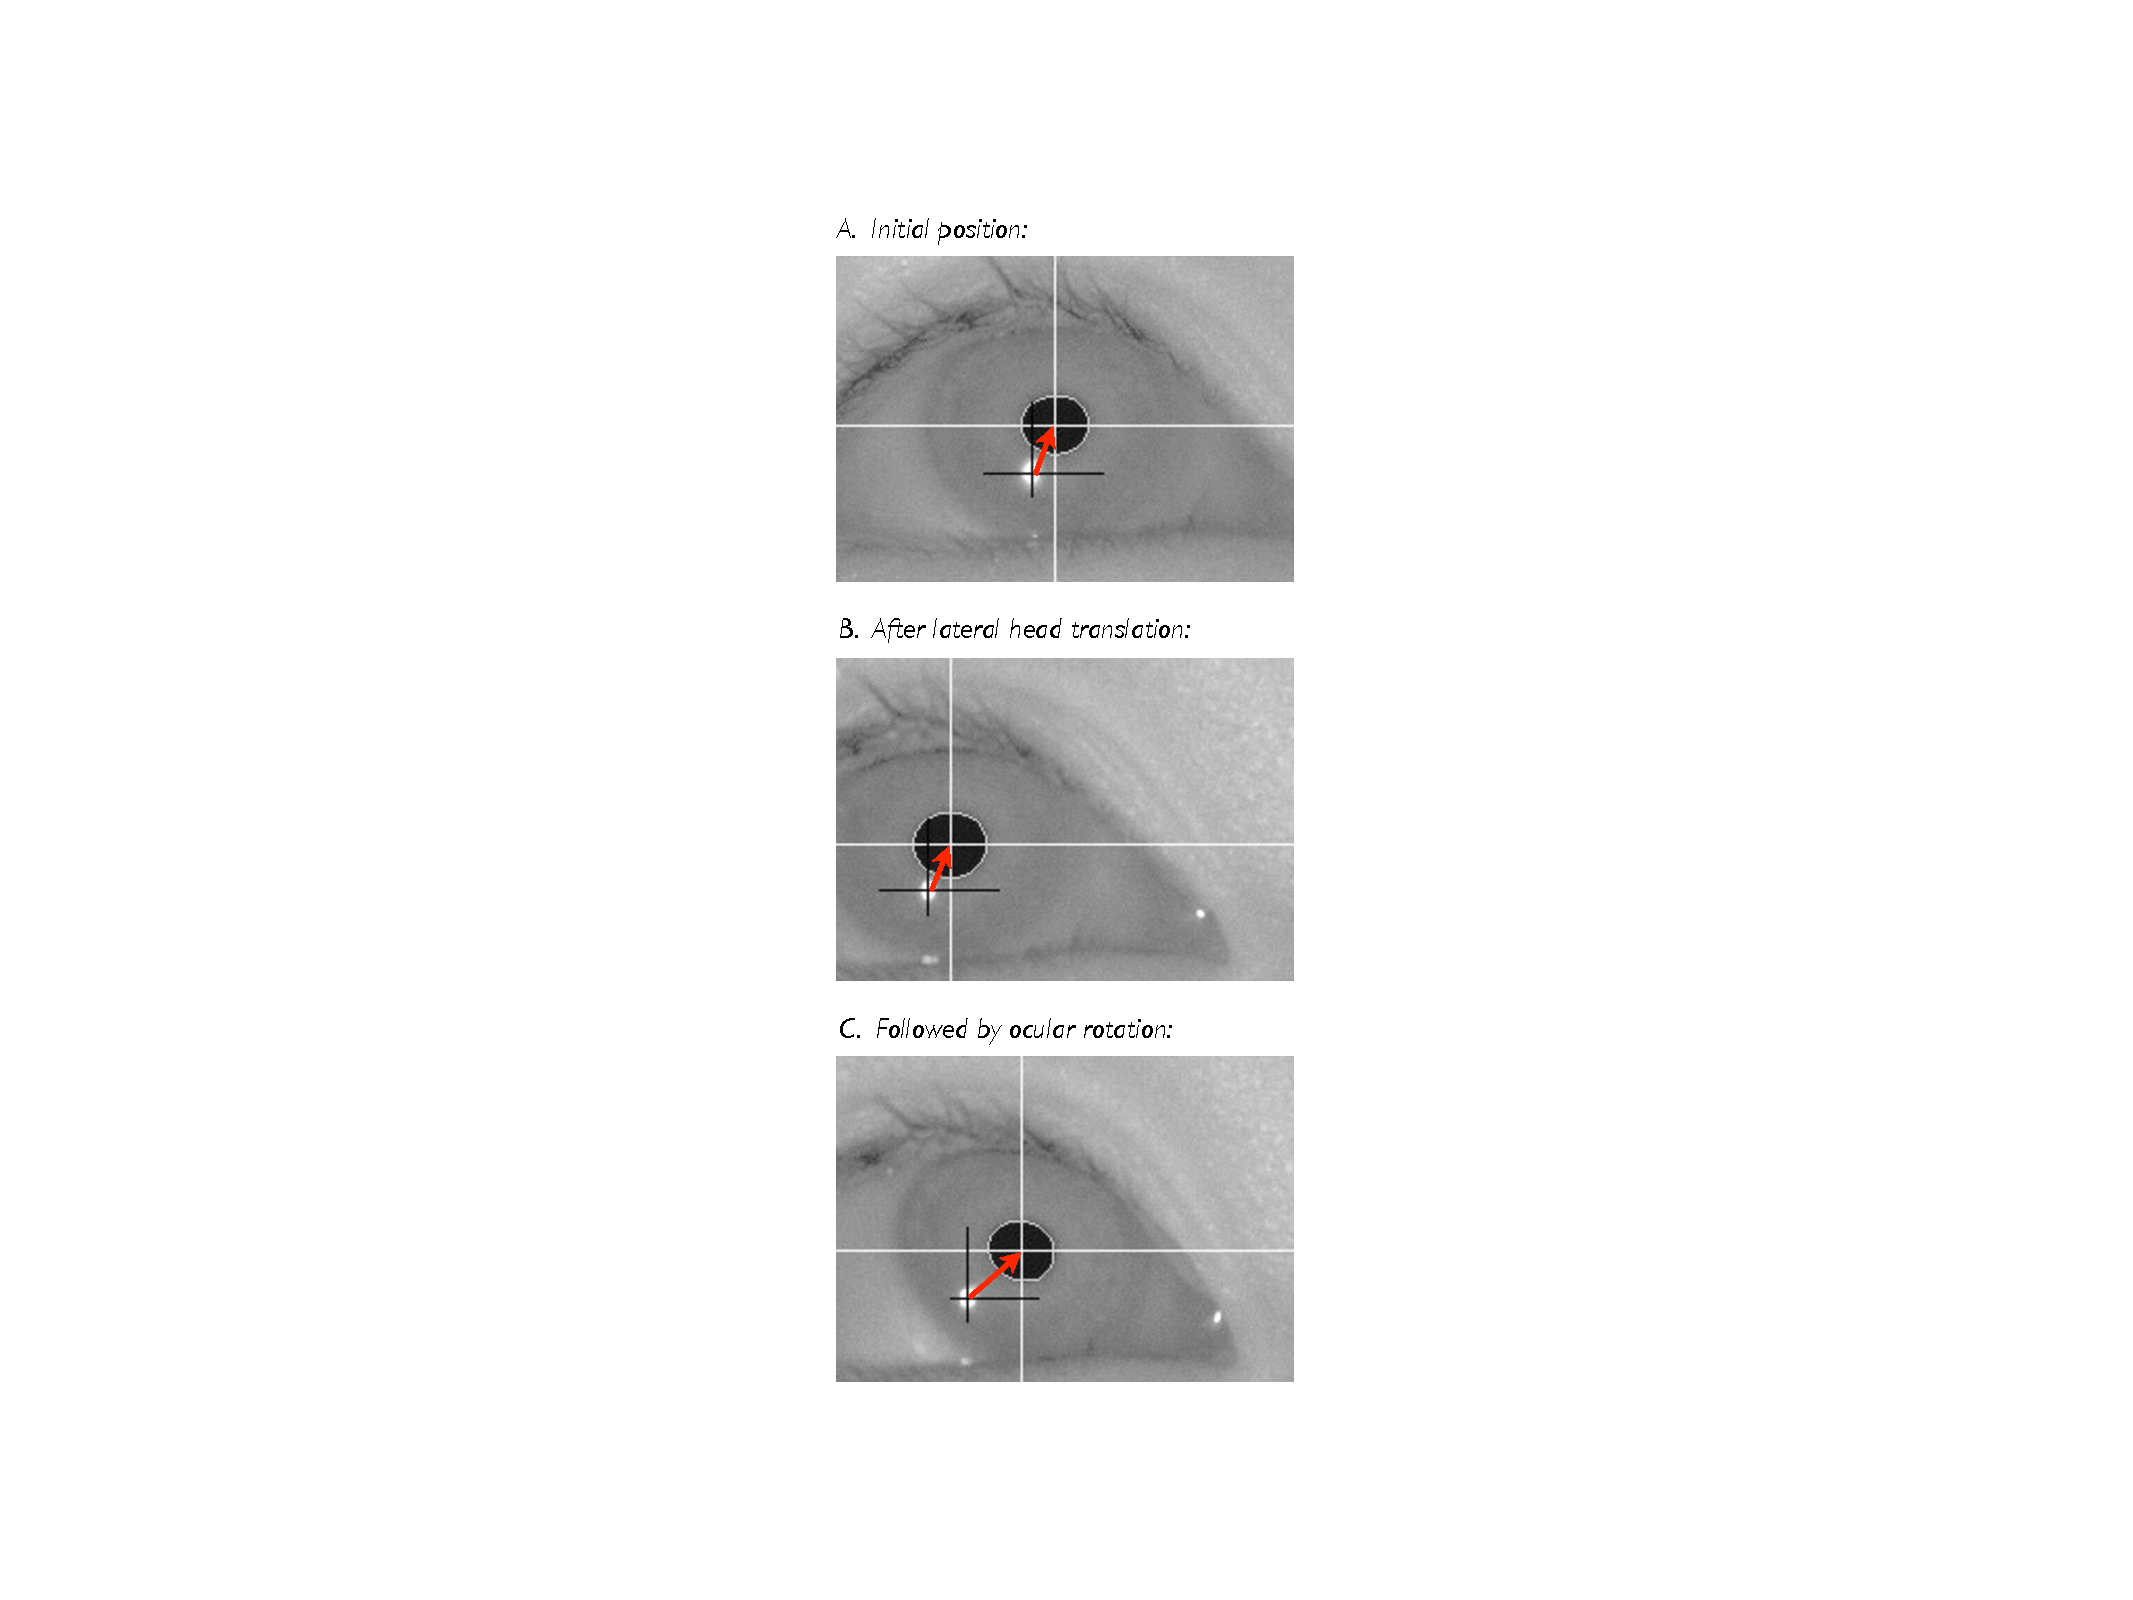
\includegraphics [width=0.70\textwidth]{Figures/Figure_1_Explanatory}
\caption{The position of the pupil within a camera image can vary due to either rotation of the eye within the head or to displacement of the head relative to the camera. Here we show how corneal reflection-stabilised pupil tracking can resolve this ambiguity. The left column shows still images taken from the eye tracker used in this study. In the right column, the simple physical model of a pool ball demonstrates the same optical principles. \textbf{\textit{(A)}} The eye tracker has identified the pupil and the first Purkinje reflection from the corneal surface, each indicated by cross-hairs. The red arrow is the vector of their relative position. The corneal reflection is due to a light source transmitted from a mirror below the eye, and hence appears below the pupil. On the pool ball, the figure 8 represents the pupil and the white stripes are the reflection of fluorescent lights on the ceiling above. \textbf{\textit{(B)}} The subject has deliberately displaced his head horizontally relative to the camera, while maintaining gaze on a centrally-located visual target. Both the pupil and the corneal reflex have shifted considerably within the video image. Their relative position, however, as indicated by the red arrow, is unchanged. The same is true following horizontal displacement of the pool ball relative to a fixed camera. In this case, the calibrated eye tracker would show that gaze position was stable, despite the substantial shift of the pupil within the image. \textbf{\textit{(C)}} The head remains stationary at its new location while the eye rotates nasally within the orbit. The pupil centre and corneal reflex have moved differentially, as shown by the red arrow (note that for the perfectly spherical pool ball, the surface reflection does not move at all under pure rotation). By tracking the pupil-reflection relative position vector rather than the raw pupil signal, the eye tracker can yield a signal that reflects pure gaze change, without artefacts due to head motion relative to the camera.}
\label{fig:PCCR}
\end{center}
\end{figure*}

\section{Methods}

\subsection{Subjects}

Data came from an ongoing variable-endpoint longitudinal study at the New Zealand Brain Research Institute, Christchurch, New Zealand. We examined 188 patients (69\% male), with mean age 68.3 years (\textit{SD} 8.4), mean symptom duration 8.2 years (\textit{SD} 5.0), mean MDS-UPDRS part III score 33.4 (\textit{SD} 16.9) and mean Hoehn \& Yahr score 2.3 (\textit{SD} 0.7). The 66 controls (64\% male) had a mean age of 70.3 (\textit{SD} 8.5). Participants were assessed from 1-7 times (mean 2.7) over an eight year period, for a total of 491 Parkinson's and 190 control sessions. We utilised data from each visit, but the conclusions remained the same if we restricted the analysis to just one recording per person. 

A movement disorders specialist (TJA) confirmed that patients met the UK Brain Bank criteria for idiopathic Parkinson's \citep{Hughes1992Accuracy-of-cli}. Exclusion criteria were previous history of other neurological, psychological or medical conditions, including atypical Parkinson's disease; moderate or severe head injury, stroke, major depression or learning disability; a history of cranial neurosurgery; major heart disease; diabetes requiring insulin; and alcohol abuse. The study was approved by the Ethics Committee of the New Zealand Health and Disability Commission. All subjects gave written consent and caregivers provided additional consent for participants with significant cognitive impairment.

\subsection{Apparatus}
Eye movements were recorded with an iView X Hi-Speed (SMI, Berlin), an infrared pupil and corneal reflection video tracking system which acquired samples monocularly at 1250 Hz (usually from the left eye). Participants were seated, with forehead and chin resting upon the eye tracker column. Although participants were encouraged to keep as still as possible during recordings, the head was not physically restrained.

\subsection{Procedure}
Participants performed a range of oculomotor saccadic tasks in response to a jumping red square target. Only data from the first, simple visually-guided task is presented here, as it is similar to the task reported by \cite{Gitchel2012Pervasive-ocula}. Our task has been fully described previously \citep{MacAskill2012The-influence-o}, in an earlier overlapping cross-sectional sample of 163 patients and 48 controls.
In essence, the target (subtending 0.75 deg) jumped at inter-stimulus intervals ranging from 550 to 1800 ms, moving purely horizontally by pseudo-random steps of 5, 10, 15 or 20 deg leftwards or rightwards. The new target position was constrained to always remain within 15 deg of centre and served as the fixation point for the next trial. The task duration was 121 s, comprising 108 target steps.

\subsection{Data processing}
Data processing and analysis was performed in the \textit{Python} programming language (version 2.7.8) using the packages \textit{numpy} (1.9.1) and \textit{scipy} (0.14.0). Raw horizontal and vertical coordinates of the centroids of the pupil and the corneal reflection were determined within each $224 \times 160$ pixel video frame by the manufacturer's algorithm. We isolated periods of fixation by deleting sections where a saccade was present (aggressively defined as intervals in the pupil centre signal in which the velocity exceeded 150 pixels per second, with the resulting window extended by 20 ms before and after). These parameter values were shown by visual inspection to effectively exclude saccades while retaining periods of fixation. Regions where tracking was lost (such as during blinks) were excluded.

The resulting pupil and corneal reflection signals from the fixation periods were filtered and down-sampled (decimated) to 125 Hz using a 30 point finite impulse response filter with a Hamming window to eliminate high-frequency noise. This reduced the maximum detectable frequency to 62.5 Hz, well above our expected maximum frequency of 30 Hz for any tremor of mechanical or neurogenic origins. Subtracting the decimated corneal reflection signal from the decimated pupil signal generated the reflection-corrected signal. The gradients of the pupil, reflection, and reflection-corrected signals were then calculated using central differences in the interior and first differences at the boundaries. This removed the constant offsets due to the differing gaze angles across fixations. We used principal component analysis to determine the axis of primary variability (horizontal, vertical, or oblique) in the pupil gradient data.

The power spectra of the entire decimated, differentiated, and projected pupil, reflection, and reflection-corrected signals for each subject were then determined by fast Fourier transforms, with a window size of 1024 samples and an overlap of 512 samples (equating to a moving window of 8.2 s with an overlap of 4.1 s). For each subject, a mean power spectrum across windows was produced for each of the three signals. The spectrum was then corrected for the scaling caused by differentiating the signal, and multiplied by the frequency response of a band-pass Butterworth filter (5th order, low cut-off of 1.0 Hz, high cut-off of 40 Hz) to remove the DC component. From each spectrum, the power value at the highest peak (i.e. the maximum power) was determined, along with the frequency at which it occurred.

This analysis was designed to be fully reproducible, with analysis code and raw data made open and publicly available under a Creative Commons CC BY-SA 3.0 license. \textbf{See http://nzbri.org/eyelab/ for links to code and raw data.}

\subsection{Statistical analysis}
Our primary quantitative results (Figures \ref{fig:FFT} -- \ref{fig:main}) are presented without accompanying inferential statistics. The intention was to show that a feature in one signal either is or is not abolished by subtracting another signal from it. Sample variability is not a credible explanation for an effect of the resulting magnitude. That is, meaningful alternative explanations would need to be mechanistic rather than probabilistic.

To assess any correlation between eye signal oscillation power and clinical somatomotor tremor severity, we used a linear mixed effects model to account for the fact that we  Figure \ref{fig:UPDRS}

\section{Results}
Principal component analysis revealed that the primary direction of any pupil signal oscillation was close to the horizontal for nearly all patients and controls. The following results are therefore based on analysis of the horizontal component of the data. Brief extracts from four representative Parkinson's recordings are shown in Figure \ref{fig:traces}. Apparent pupil signal oscillations ranged from striking (Figure \ref{fig:traces}A, \ref{fig:traces}B), with obvious head motion at the time of recording, to subtle (Figure \ref{fig:traces}C, \ref{fig:traces}D). Regardless, all four corrected signals (the difference between the raw pupil and corneal reflex signals) show no apparent oscillation. That is, pupil centre-corneal reflection subtraction is clearly effective at removing head movement artefacts.

\begin{figure*}[htbp]
\begin{center}
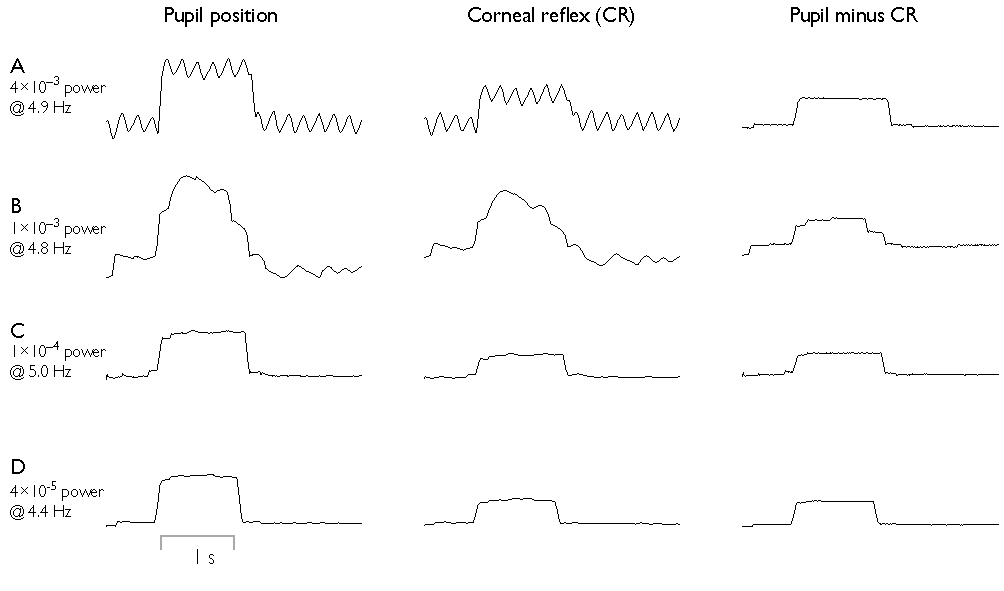
\includegraphics {Figures/Figure_2_Individual_traces}
\caption{Representative eye tracking signals from four Parkinson's participants who fell in the putative range of ``ocular tremor'' frequency in their raw pupil signal (\textasciitilde{}3 s of data as the eyes tracked a target which stepped 20 deg rightwards and then leftwards). The first column shows the raw position of the centre of the pupil within the camera image, while the second shows the position of the corneal reflection. The final column shows the difference between the two signals. Varying signal amplitudes across the subjects reflect that these are raw, uncalibrated data. \textbf{\textit{(A, B):}} These participants had upper limb tremor which was transmitted to the head, causing a major head motion artefacts in both the raw pupil and corneal reflection signals. \textbf{\textit{(C, D):}} These participants had much lower peak power in their raw signals, with any oscillation being much more subtle.
The effectiveness of simply taking the difference between the two raw signals is shown in the right-most column, in which head motion artefacts are eliminated. All four corrected signals show similarly stable gaze fixations, despite the striking range of head motion across subjects.
}
\label{fig:traces}
\end{center}
\end{figure*}

Figure \ref{fig:FFT} reveals the key finding graphically, showing the power spectrum of each recording's fixation periods, derived from the Fourier transform of each signal. There were clear peaks in the somatomotor tremor frequency range in both the raw pupil and corneal reflex signals. These peaks were common and prominent in the Parkinson's group and also occurred, although less commonly and at lower magnitude, in the control group. These peaks were entirely abolished in the corneal reflection-corrected data (Figure \ref{fig:FFT}, right-most column). This indicates that the peaks in the raw signals were due to a common oscillation, which, given the principles illustrated in Figure \ref{fig:PCCR}, must have been due to head motion.

\begin{figure*}[htbp]
\begin{center}
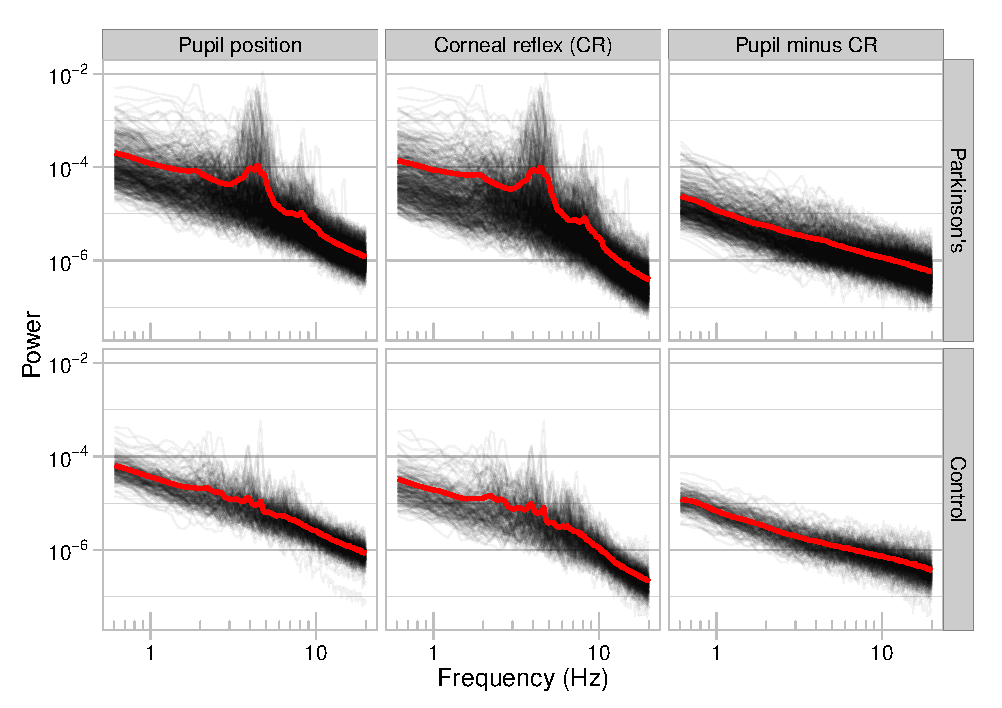
\includegraphics {Figures/Figure_3_Individual_FFTs}
\caption{For every session, we applied a fast Fourier transform (FFT) to reveal the frequency content of its pupil, corneal reflex, and pupil-minus-corneal-reflex signals (black lines). Red lines show the mean FFT for each signal in the Parkinson's (top panels) and Control groups (bottom panels). There is clear evidence of a peak in the vicinity of somatic tremor (~4 Hz) in the pupil signals from the Parkinson's group. A similar peak occurs in the corneal reflex signal. It is completely abolished in the signal formed by simply subtracting the corneal reflex from the pupil signal (right-most panels). This indicates that the oscillation was common to the two signals, and hence due to head motion. A similar pattern was seen in the controls, where a small number of participants also showed peaks in the somatic tremor range. The 4 Hz activity in the pupil data is likely to be the same oscillation reported by Gitchel et al. That is abolished when correcting with the corneal reflex signal indicates that it is an artefact of head motion rather than an oscillation of intrinsically ocular origin.}
\label{fig:FFT}
\end{center}
\end{figure*}

To more clearly depict individual-level data, from each of the FFTs depicted in Figure \ref{fig:FFT} we determined, for every recording from each participant, the peak power of each of their three signals (raw pupil position, corneal reflex position, and the difference between them) and the frequency at which that peak occurred (Figure \ref{fig:main}). This corresponds to the findings of \citet{Gitchel2012Pervasive-ocula}, in that the distribution of the maximum power of the pupil signal in Parkinson's participants showed a clear peak within the grey region of Figure \ref{fig:main} (representing Gitchel et al.'s reported tremor range of 5.7 $\pm$ 3 Hz). The distribution of peak frequencies across the patients in our data was, however, multimodal, showing that  oscillation in that frequency band was not universal. The distribution of frequencies was similar in the controls (see the histograms along the $x$ axes of Figure \ref{fig:main}). The distribution of oscillation power (on the $y$ axis) was clearly different, however, with controls clustering at lower values, presumably indicating the lower amplitude of any somatomotor tremor in that group.

\begin{figure*}[htbp]
\begin{center}
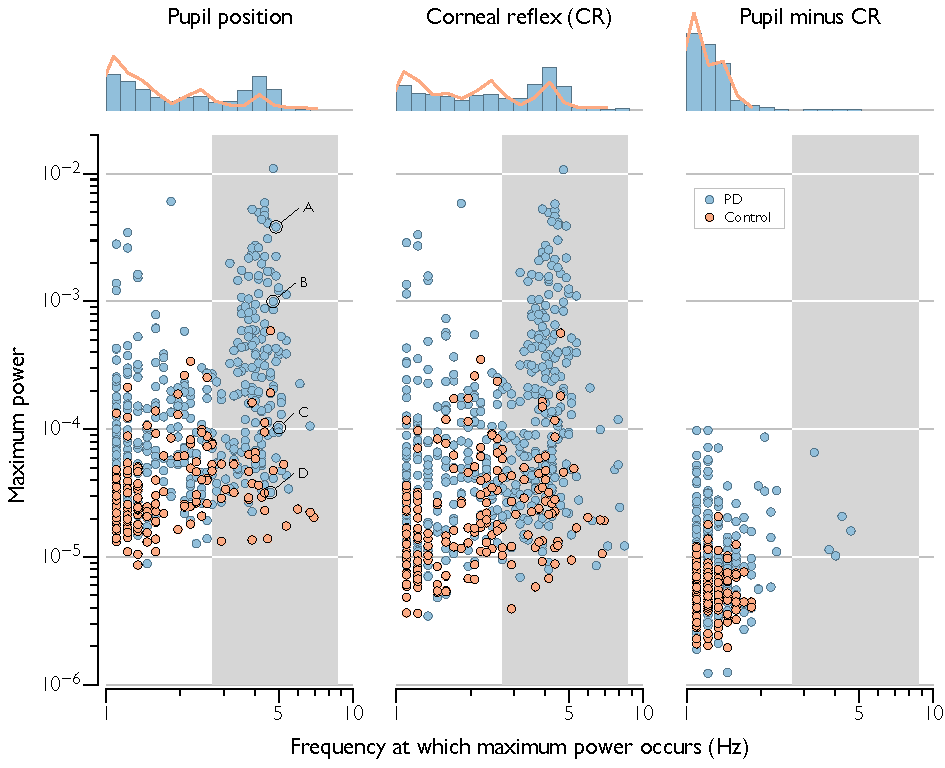
\includegraphics {Figures/Figure_4_Main_frequency_data}
\caption{For each session, a Fast Fourier Transform was applied to data from the ocular fixation periods (see Figure \ref{fig:FFT}). Points represent the peak power in each signal (left panel = raw pupil position, middle = raw corneal reflex position, right = the difference between the two) and the frequency at which it occurred. Blue points = PD, orange = Control. The labelled points \textbf{\textit{(A-D)}} correspond to the selected recordings shown in Figure \ref{fig:traces}. For reference, the grey rectangular regions represent the mean tremor frequency $\pm$ 2\textit{SD} (5.7 $\pm$ 3 Hz) reported by \cite{Gitchel2012Pervasive-ocula}. The histograms (top) reveal that one of several modes for maximum power occurs at approximately 4 Hz in the pupil and corneal reflex signals, in both the patients and controls. Although the frequency distribution ($x$ axis) was similar across the groups, the power distribution ($y$ axis) shows that the strongest oscillations were more common in PD (on re-examination, the control with the highest power value was found to have a bilateral arm tremor of non extra-pyramidal origin). In the difference signal (i.e. pupil minus corneal reflex), the peak near 4 Hz was effectively abolished, with the distribution becoming dominated by what may be low frequency drift. That is, when head motion was corrected for by subtracting the corneal reflex signal from the pupil signal, the direction of gaze remained stable in space. This is strong evidence that there was no purely ocular tremor in either the Parkinson's cases or controls.}
\label{fig:main}
\end{center}
\end{figure*}

The middle panel of Figure \ref{fig:main} shows information not measured by Gitchel et al.: the peak power and oscillation frequency of the corneal reflection signal. It can be seen that its distribution in both dimensions is almost identical to the pupil data. That is, both signals appear to exhibit the same frequency and power properties. The right-most panel of Figure \ref{fig:main} shows values from the signal formed by subtracting the corneal reflection signal from the pupil signal. As in Figure \ref{fig:FFT}, any common oscillation was removed by the subtraction and we see that just five recordings had peak values which remained within the proposed tremor frequency range (the grey region), albeit at only low power.

The abolition of the putative ``tremulous'' oscillation signal following corneal reflection correction suggests strongly that it was indeed secondary to head motion. We therefore expected some relationship between the clinically-rated severity of somatomotor tremor (as assessed by the sum of the MDS-UPDRS tremor item scores) and any oscillation in the pupil and corneal reflection signals. Given the effectiveness of the corneal reflection stabilisation, we expected little to no relationship with the difference signal. Each of these predictions was supported by the data, as shown in Figure \ref{fig:UPDRS}.

\begin{figure*}[htbp]
\begin{center}
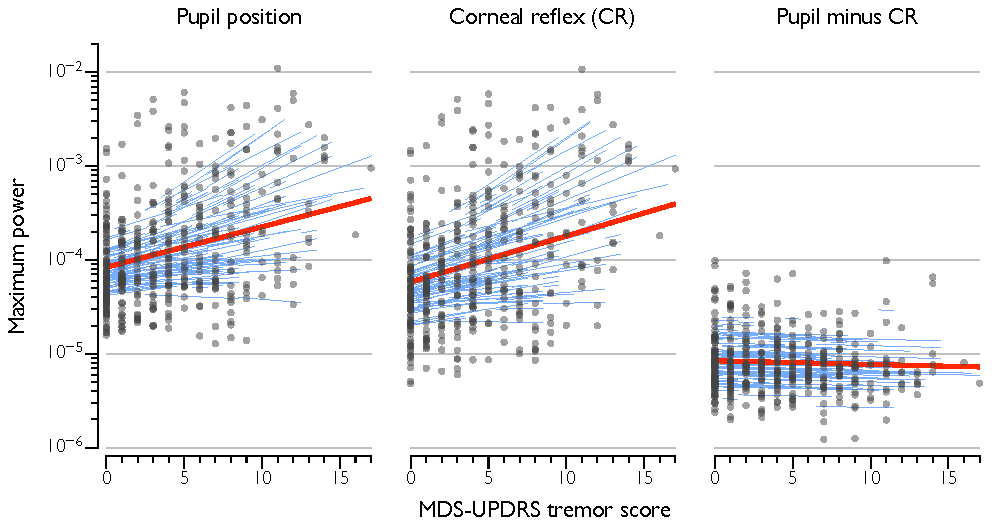
\includegraphics {Figures/Figure_5_UPDRS_correlation}
\caption{Circumstantial evidence that the apparent oscillation in ocular signals was due to somatomotor tremor. Across 186 patients for whom at least one UPDRS assessment was available, the strength of the apparent oscillation in both the pupil and corneal reflex signals was positively related logarithmically to the severity of somatomotor tremor (assessed as the sum of the 10 tremor items in the MDS-UPDRS, with a maximum score of 40). No such relationship was evident in the corneal reflex-stabilised signal (rightmost panel). A linear mixed effects model accounted for the repeated assessments in many of the patients.
}
\label{fig:UPDRS}
\end{center}
\end{figure*}


\section{Discussion}
We present compelling evidence that the proposed ocular diagnostic sign for Parkinson's \citep{Gitchel2012Pervasive-ocula} is simply an artefact of head motion. We found that an oscillation was indeed often present in raw pupil position signals of people with Parkinson's, at a frequency similar to that of parkinsonian somatic tremor. When corneal reflection stabilisation was applied to correct for head motion, however, that apparent tremulousness was entirely abolished (Figures \ref{fig:traces}, \ref{fig:FFT}, \ref{fig:main}). Lastly, we showed that oscillatory power in the pupil and corneal reflex signals was strongly correlated with the clinical severity of somatomotor tremor. No such relationship existed in the head-motion corrected signal (Figure \ref{fig:UPDRS}). Our study was, therefore, not a failure to replicate the original finding. Rather, it is a direct refutation: we detected a pupil oscillation with similar characteristics to that described by Gitchel et al. but also demonstrated that it was not purely ocular in origin.

\citet{Gitchel2012Pervasive-ocula} recognised that head motion was an obvious alternative explanation for their findings. In a subset of 62 of their original patients, they therefore used magnetic tracking apparatus to measure head oscillation and did not detect any. We, and others, have pointed out that their system is not suited to detection of such low-amplitude oscillations due to the filtering it applies \citep{MacAskill2013Ocular-Tremor-i,Saifee2014Tremor-of-the-e}. In our experience, it is highly unlikely that not a single patient in such a large sample would have a clinically-evident degree of head motion. That none was detected quantitatively seems to us to much more likely indicate insensitivity of the measuring equipment rather than the universal absence of head motion. Conversely, if a purely ocular oscillation had the claimed characteristics, it would be observed routinely during ophthalmoscopy \citep{Leigh2013Tremor-of-the-e,Saifee2014Tremor-of-the-e} and would, therfore, likely have been initially reported in the nineteenth rather than twenty first century.

Can the conflict between our findings and those of Gitchel et al. be due to eye tracking hardware differences? Our SMI column-based eye tracker provides chin and forehead rests, with no physical restraint upon the subject. A person with head motion is therefore able to move much more relative to the camera than when wearing an EyeLink, in which the cameras are attached to a headband. Using the SMI system was therefore conservative with respect to disproving the ocular tremor hypothesis. With the head unrestrained relative to the camera, apparent pupil oscillation due to head motion will be potentially much larger than in a headband-mounted tracker. If the corneal reflection correction was not highly effective, we were actually at greater risk of detecting a residual (artefactual) oscillation in the stabilised signal than if we had been using a head-mounted system. 

One difference between our findings that might be explained by equipment differences was the dominant direction of the pupil oscillation. In our data, it was primarily horizontal (according with our visual observations of the eye image during recordings of people with noticeable somatomotor tremor) whereas for Gitchel et al. it was primarily vertical. This may reflect that the head is free to move relative to the world when wearing the EyeLink system, whereas with the column-mounted chin and forehead rests of the SMI, natural vertical head motion is somewhat inhibited and perhaps is more naturally expressed horizontally due to those physical constraints.

\citet{Gitchel2012Pervasive-ocula} stated that all patients showed ``oscillatory behaviour'' while all but two controls showed ``highly stable fixations''. No threshold values for making these judgments were stated and there is an implication that they were not judged by the same criteria. Quantitative Fourier transforms were said to have been applied ``in cases of fixation instability'' rather than to all recordings. Whatever the basis of this pre-selection of cases, it apparently resulted in an FFT being applied to all patients but only two controls. No quantitative measurements were presented of any oscillations which may have been present in the other 58 controls. By contrast, we analysed every recording quantitatively. We found the distribution of the dominant oscillation frequencies to be similar between patients and controls (Figure \ref{fig:main}, $x$ axis) although the amplitudes of those oscillations were in general higher in the patients (Figure \ref{fig:main}, $y$ axis). Pre-selecting recordings by subjectively identifying cases with ``fixation instability'' would, therefore, tend to exclude actual oscillations in control data simply because, when present, they will likely be of very small amplitude.

When present, the similar frequencies of the head-motion related oscillations in the controls and patients in our study is itself interesting. It suggests that small-amplitude somatomotor tremor, near the characteristic frequency generally ascribed to Parkinson's, is not uncommon in healthy older adults. This indicates that video-oculography may be indirectly sensitive to signs of subtle, sub-clinical somatomotor tremor \citep{MacAskill2013Ocular-Tremor-i}.  (\citet{Shulman1996Internal-tremor} found that diagnosed patients themselves frequently report a sensation of ``internal tremor'', prior to the development of clinically-evident shaking.)  It is also supportive of the characteristic rest tremor of Parkinson's being an amplification of a normal phenomenon. That is, although Parkinson's rest tremor might arise as a de novo pathological oscillation \citep{McAuley2000Physiological-a}, it has alternatively been hypothesised that it is due to pathologically increased output from an oscillatory motor control network that drives normal voluntary rhythmical movement \citep{Burkhard:NeurophysiolClin:2002,Schnitzler2005Normal-and-path,Schnitzler2006Physiological-a}, and there are thalamo-cortical-thalamic motor circuits with a natural resonance frequency of 4-5 Hz \citep{Volkmann:Neurology:1996}.

The hypothesis that parkinsonian rest tremor is an amplification of a normal motor oscillation remains to be confirmed. Although we reject the existence of a diagnostic ocular oscillation in Parkinson's, oculomotor data may yet provide indirect insights into the origin of the disorder's characteristic resting somatomotor tremor.


\section{Acknowledgements}
The data came from a series of projects funded by the Canterbury Medical Research Foundation, Neurological Foundation of New Zealand, and New Zealand Brain Research Ltd.

The authors declare that there is no conflict of interest regarding the
publication of this paper.

\bibliography{ocular_tremor}

\end{document}
